\chapter{Fundamentação teórica}
%%%%%%%%%%%%%%%%%%%%%%%%%%%%%%%%%%%%%%%%%%%%%%%%%%%%%%%%%%%%%%%%%%%%%%
Neste capitulo, apresentamos uma síntese da revisão bibliográfica realizada para embasar a metodologia adotada no desenvolvimento e simulação do ADPLL. São abordados os conceitos básicos de um sintetizador de frequência, o protocolo de comunicação \textit{Bluetooth} e a importância dos circuitos e dispositivos CMOS. Esses tópicos são fundamentais para compreender o funcionamento do ADPLL e sua aplicação em sistemas de comunicação sem fio. A revisão bibliográfica oferece uma base sólida para o desenvolvimento do projeto, fornecendo os conhecimentos necessários para explorar as características, desempenho e aplicações do ADPLL.

%%%%%%%%%%%%%%%%%%%%%%%%%%%%%%%%%%%%%%%%%%%%%%%%%%%%%%%%%%%%%%%%%%%%%%
\section{Sintetizador de frequência}
%%%%%%%%%%%%%%%%%%%%%%%%%%%%%%%%%%%%%%%%%%%%%%%%%%%%%%%%%%%%%%%%%%%%%%
Em sistemas de comunicação sem fio a presença de um circuito sintetizador de frequência é essencial. O circuito sintetizador de frequência é responsável por gerar a frequência central de um canal em um sistema de comunicação de Rádio Frequência (RF). Cada canal possui uma faixa de frequência especifica de operação, desta forma o circuito do Sintetizador deve ser capaz de permitir ajustes de frequência pequenos.

O circuito Sintetizador de frequência gera as frequências necessária como um múltiplo de uma referência do Oscilador de Cristal Controlado por Temperatura (TXCO, do inglês \textit{Temperature-Controlled Crystal Oscillator}). O TXCO papel fundamental na performance do sintetizador, é responsavél por fornece uma frequência estável e precisa e com baixo valor de ruido de fase. De acordo com \cite{lascari2000accurate} negligenciar seus efeitos em um sintetizador pode acarretar em resultados inesperados após a concepção do circuito.

O processo de síntese de frequência ocorre através de técnicas de geração e mistura de sinais. Primeiramente, a referência de TXCO fornece uma frequência estável e precisa. Em seguida, o sintetizador de frequência utiliza circuitos internos, como divisores de frequência e circuitos de fase, para manipular e multiplicar a frequência da referência, produzindo assim a frequência desejada.


%%%%%%%%%%%%%%%%%%%%%%%%%%%%%%%%%%%%%%%%%%%%%%%%%%%%%%%%%%%%%%%%%%%%%%
\section{PLL}
%%%%%%%%%%%%%%%%%%%%%%%%%%%%%%%%%%%%%%%%%%%%%%%%%%%%%%%%%%%%%%%%%%%%%%
PLL (\textit{Phase-Locked-Lopp}) é um circuito Sintetizador de frequência comumente utilizado. PLL é composto por diversos blocos, alguns deles são: osciladores controlados por tensão VCO (\textit{Voltage-Controlled Oscillator}), divisores programáveis, comparadores de fase DFF (Detectores de Fase e Frequência), bombas de carga CP (\textit{Charge Pump}) e Filtros Passa Baixas LPF (\textit{Low Pass Filters}). 

Os blocos que compõem um PLL são apresentados na Figura \ref{fig:pll_blocks}.
A utilização de uma realimentação negativa no circuito permite um controle tanto de frequência como de fase para a saída.

\begin{figure}[h!]
	\caption{Diagrama de blocos de um PLL.}
	\begin{center}
		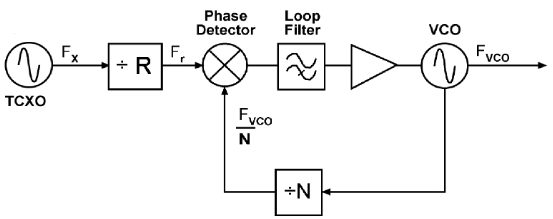
\includegraphics[scale=0.6]{img/pll_blocos.png}
	\end{center}
	\fonte{\citeonline{barrett_1999_fractionalintegern}}
	\label{fig:pll_blocks}
\end{figure}

O PLL utiliza o VCO como elemento central. O sinal de saída do VCO, dividido por um fator N, é comparado com a frequência de referência do TXCO, dividida por R, pelo  \textit{Phase-Detector}. Após a comparação, o sinal resultante passa pelo\textit{Loop filter}, responsável por eliminar ruídos e interferências. A saída do \textit{Loop filter} é uma tensão que controla a tensão aplicada ao VCO, permitindo ajustar e manter a frequência de saída em sincronia com a frequência de referência \cite{barrett_1999_fractionalintegern}.

Em condições normais, um PLL fornece uma frequência com extrema precisão, no entanto, o tempo de aquisição pode ser longo devido ao processo do detector de fase e frequência em avaliar e gerar sinais com base nas diferenças em relação à referência. Esse tempo de aquisição é especialmente crucial em aplicações de comunicações sem fio que envolvem técnicas como salto de canal (\textit{frequency hopping}), como é o caso do protocolo \textit{Bluetooth}. Nessas situações, a capacidade do PLL de se sincronizar rapidamente com frequências variáveis é essencial para garantir uma transição suave entre os canais e evitar perdas de dados ou conexão.
%%%%%%%%%%%%%%%%%%%%%%%%%%%%%%%%%%%%%%%%%%%%%%%%%%%%%%%%%%%%%%%%%%%%%%
\subsection{Integer-N PLL}
%%%%%%%%%%%%%%%%%%%%%%%%%%%%%%%%%%%%%%%%%%%%%%%%%%%%%%%%%%%%%%%%%%%%%%

PLLs convencionais também conhecidos como \textit{Integer-N PLL} são capazes de gerar apenas frequências de valores N vezes a frequência do TXCO, onde N é um valor inteiro, desta forma a resolução de frequência é definida pela frequência de referência utilizada. 

A frequência de saída é definida como:

\begin{equation}
	F_{VCO} = N \cdot F_{ref}
	\label{eq:fvco_integer_PLL}
\end{equation}



%%%%%%%%%%%%%%%%%%%%%%%%%%%%%%%%%%%%%%%%%%%%%%%%%%%%%%%%%%%%%%%%%%%%%%
\subsection{Fractional-N PLL}
%%%%%%%%%%%%%%%%%%%%%%%%%%%%%%%%%%%%%%%%%%%%%%%%%%%%%%%%%%%%%%%%%%%%%%
Em um \textit{fractional-N} PLL a frequência de saída pode ser ajustada como uma fração da frequência de referência. Esse ajuste fracional é necessário em sistemas de comunicação para o ajuste correto da frequência central de canal utilizado. 

\textit{Fractional-N} PLL utiliza uma topologia similar ao do \textit{Integer-N} PLL, com adição de um acumulador, uma maquina de alterna o divisor entre (N e N+1) durante um estado bloqueado. Esta variação faz com que a média torne-se um valor fracional entre N e N+1, proporcionando um ajuste de frequência também fracional. 

A frequência de saída é definida como:

\begin{equation}
	F_{VCO} = (N + F) \cdot F_{ref}
	\label{eq:fvco_fractional_PLL}
\end{equation}
Onde, $F$ é $0$ ou $1$. 

%%%%%%%%%%%%%%%%%%%%%%%%%%%%%%%%%%%%%%%%%%%%%%%%%%%%%%%%%%%%%%%%%%%%%%
\section{ADPLL}
%%%%%%%%%%%%%%%%%%%%%%%%%%%%%%%%%%%%%%%%%%%%%%%%%%%%%%%%%%%%%%%%%%%%%%
%O ADPLL \textit{All Digital Phase-Locked-Loop} é um circuito Sintetizador de frequência que ao contrário dos PLLs convencionais é um puramente digital. Em um PLL tradicional o \textit{Loop-Filter} ocupa mais de 50\% da área do chip, enquanto que no ADPLL por ser um circuito digital não necessita de grandes componentes, capacitores, resistores e indutores, reduzindo em grande parte a área ocupada.
%
%A utilização de circuito digital se da devido a miniaturização da tecnologia CMOS, permitindo maiores velocidades, maiores frequências, e assim, propiciando o uso de \textit{design} de circuitos digitais em RF. Seu uso traz inúmeros benefícios, entre elas a possibilidade de parametrização do \textit{Loop-Filter} para ajuste de frequência conforme desejado, e sendo o ADPLL totalmente digital não necessita circuitos auxiliar de conversão do sinal digital para analógico ou vice-versa, sendo uma grande vantagem.


O ADPLL (\textit{All Digital Phase-Locked-Loop}) é um sintetizador de frequência que se diferencia dos PLLs convencionais por ser um circuito puramente digital. Enquanto um PLL tradicional requer componentes analógicos, como capacitores, resistores e indutores, o ADPLL aproveita os benefícios da miniaturização da tecnologia CMOS, permitindo maiores velocidades e frequências, além de reduzir significativamente a área ocupada no chip.

Para \cite{staszewski2006all} a tecnologia nanométrica do CMOS traz um novo paradigma, a resolução do domínio do tempo de uma transição de borda de sinal digital é superior à resolução de tensão de sinais analógicos. Desta forma o ADPLL pode ser analisado apenas pelas transições dos sinais digitais.

A natureza digital do ADPLL oferece vantagens adicionais, como a parametrização do \textit{Loop-Filter} para ajuste de frequência conforme necessário. Além disso, não são necessários circuitos auxiliares para conversão entre sinais digitais e analógicos, o que representa uma economia de recursos e simplificação do projeto.

%Tanto uma onda sinusoidal quanto uma onda retangular podem ser utilizadas como a frequência de referência do circuito. No entanto, é comum usar uma onda retangular para análise, visto que o circuito é sincronizado e controlado pelas transições do \textit{clock} de referência (FREF), proporcionando uma análise rápida e precisa do comportamento do ADPLL.

A Figura \ref{fig:adpll_block_diagram} mostra o diagrama de blocos de um ADPLL no domínio do tempo, ou seja considerando as transições dos sinais de (FREF) e saída do circuito (DCO). O ADPLL é composto de 4 blocos principais,  \textit{Digital Controlled Oscillator} (DCO), \textit{Time to Digital Converter} (TDC), \textit{Phase Detector} (PD) e o \textit{ digital Loop Filter} (LF). Nas subseções seguintes serão apresentados com mais detalhes cada um dos sub-blocos. 

\begin{figure}[h!]
	\caption{Diagrama de blocos de um ADPLL.}
	\begin{center}
		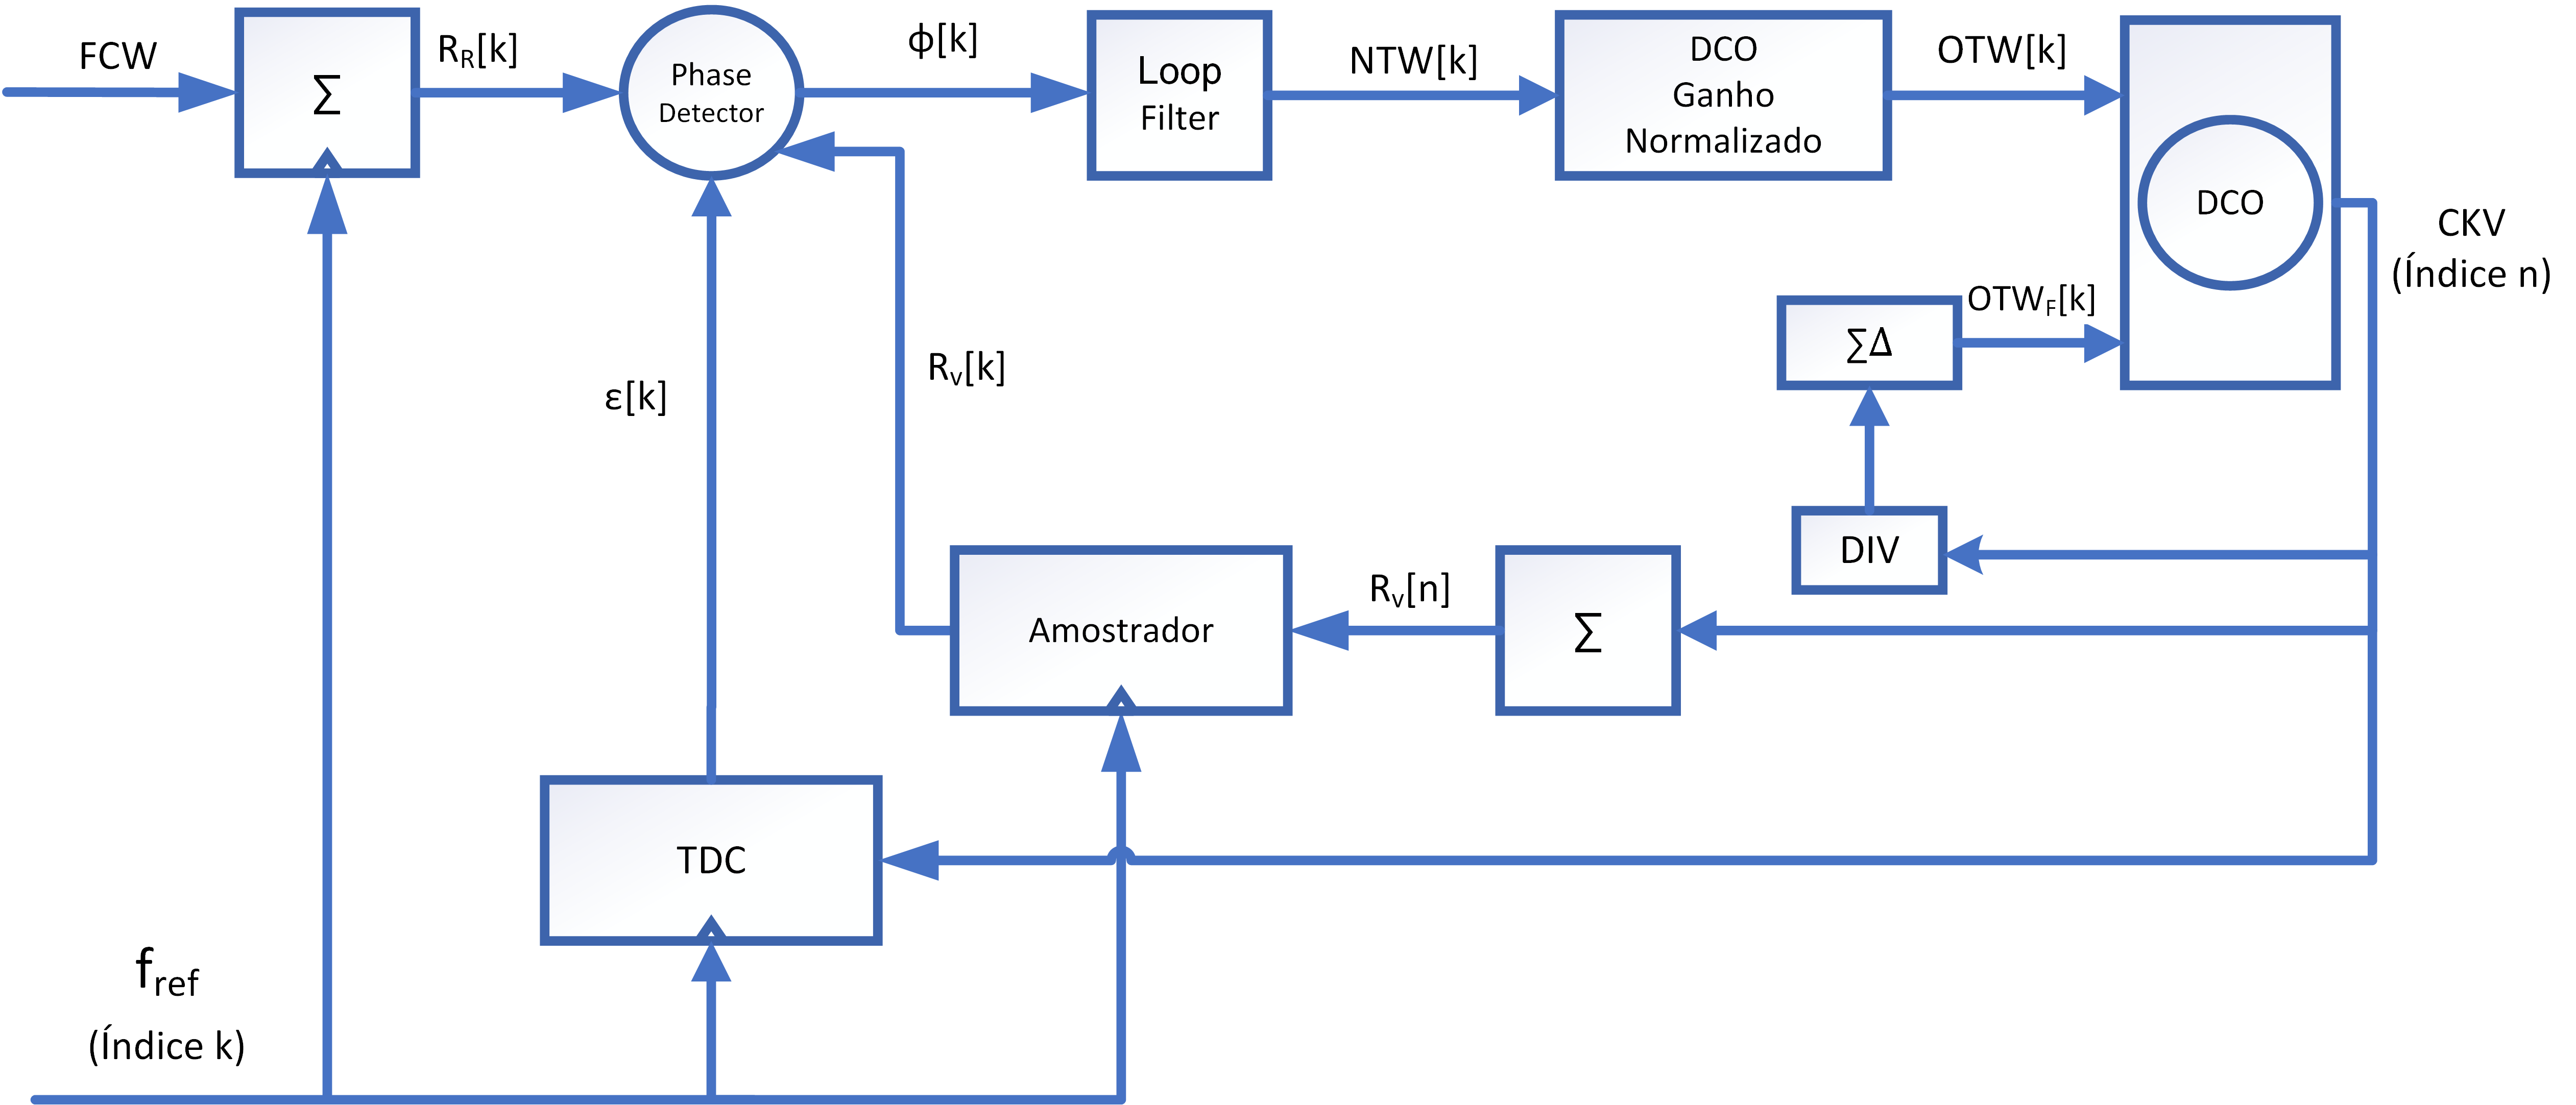
\includegraphics[scale=1]{img/blocos_ADPLL.png}
	\end{center}
%	\fonte{\citeonline{staszewski2006all}}
	\label{fig:adpll_block_diagram}
\end{figure}

O circuito do DCO é responsável por gerar o sinal de saída do sintetizador. Ele consiste em um indutor fixo e um conjunto de capacitores programáveis que formam um circuito ressonante LC. A frequência de saída é definida pelo FCW (\textit{Frequency Command Word}), pode ser um valor fracionado ou inteiro da frequência de referência, conforme expresso na Equação \ref{eq:fvco_adpll}.

\begin{equation}
	F_{VCO} = FCW \cdot F_{ref}
	\label{eq:fvco_adpll}
\end{equation}

Por outro lado, o TDC realiza a medição da diferença de tempo entre as bordas de \textit{clock} do sinal do DCO e uma borda de referência, , acumulando esse valor a cada transição do\textit{clock}, da mesma forma que FCW. O detector de fase compara as diferenças entre os acumuladores, que é então utilizado pelo\textit{Loop Filter} para controlar os capacitores do DCO. Essa ação de controle resulta no ajuste da frequência do sinal de saída, permitindo aumentá-la ou reduzi-la conforme necessário.



%É comumente utilizado uma onda retangular para análise, na Figura \ref{fig:adpll_block_diagram}  o circuito é sincronizado e controlado pelas transições do \textit{clock} de referência (FREF), o que permite uma análise rápida e precisa do comportamento.

%Neste trabalho, optou-se por realizar uma análise focada nas transições do \textit{clock} para estudo e desenvolvimento. 


%%%%%%%%%%%%%%%%%%%%%%%%%%%%%%%%%%%%%%%%%%%%%%%%%%%%%%%%%%%%%%%%%%%%%%
%\textit{Energy Harvesting} 
%%%%%%%%%%%%%%%%%%%%%%%%%%%%%%%%%%%%%%%%%%%%%%%%%%%%%%%%%%%%%%%%%%%%%%

%%%%%%%%%%%%%%%%%%%%%%%%%%%%%%%%%%%%%%%%%%%%%%%%%%%%%%%%%%%%%%%%%%%%%%
\subsection{DCO}
%%%%%%%%%%%%%%%%%%%%%%%%%%%%%%%%%%%%%%%%%%%%%%%%%%%%%%%%%%%%%%%%%%%%%%
O DCO é o elemento principal do ADPLL, converte o \textit{Oscilator Tunning Word}, (OTW), em um sinal periódico onde a frequência $f$ é em função de sua entrada.
\begin{equation}
	f = f(OTW)
	\label{eq:f_OTW}
\end{equation}

O DCO é formado por um circuito tanque LC, um indutor fixo e um banco de capacitores programáveis, em ressonância a frequência é definida de acordo com a equação \ref{eq:f_LC} onde $C_{tot}$ é a soma de todos capacitores ativos.

\begin{equation}
	f_{out} = \frac{1}{2 \pi \sqrt{L \cdot C_{tot}}}
	\label{eq:f_LC}
\end{equation}

O DCO deve ser capaz de gerar um range de frequências e um espaçamento entre elas que atenda as especificações de modulação que será utilizado no transceptor. Para o \textit{Bluetooth } que possui um range de frequências entre $2.402GHz$ e $2.480GHz$, se utilizar 8 bits, conjunto de 256 capacitores programáveis, o passo de frequência seria $(2,480GHz - 2,402GHz)/2^8 = 304,67kHz$, o que é muito grosso para aplicações sem fio. Por outro lado se considerar um passo de frequência de $1kHz$ para a banda toda do \textit{Bluetooth }, seriam necessário 17 bits, sendo inviável de fabricação pela extrema dificuldade de casamento dos inúmeros capacitores no \textit{layout}.


A alternativa é a divisão do banco de capacitores em três partes, sendo apenas uma acionada por vez. Os modos são chamados de modo de Processo-Tensão-Temperatura  (PVT), modo de aquisição (ACQ) e modo de caminhada (TRK). Para uma boa relação entre tamanho físico e o menor passo de frequência\cite{staszewski2006all} sugere que cada banco possua 8 bits em modo PVT, 8 bits no modo ACQ e 6 bits em TRK.  O modo PVT é o primeiro ser setado, compensando as variações de processo, temperatura e tensão, centralizando o oscilador mais perto da frequência desejada, mas não exata, com variações entre $1$ a $2MHz$. 
%%%%%%%%%%%%%%%%%%%%%%%%%%%%%%%%%%%%%%%%%%%%%%%%%%%%%%%%%%%%%%%%%%%%%
\subsection{Loop Filter}
%%%%%%%%%%%%%%%%%%%%%%%%%%%%%%%%%%%%%%%%%%%%%%%%%%%%%%%%%%%%%%%%%%%%%%

%%%%%%%%%%%%%%%%%%%%%%%%%%%%%%%%%%%%%%%%%%%%%%%%%%%%%%%%%%%%%%%%%%%%%%
\subsection{TDC}
%%%%%%%%%%%%%%%%%%%%%%%%%%%%%%%%%%%%%%%%%%%%%%%%%%%%%%%%%%%%%%%%%%%%%%

%%%%%%%%%%%%%%%%%%%%%%%%%%%%%%%%%%%%%%%%%%%%%%%%%%%%%%%%%%%%%%%%%%%%%%
\subsection{Ruído de Fase}
%%%%%%%%%%%%%%%%%%%%%%%%%%%%%%%%%%%%%%%%%%%%%%%%%%%%%%%%%%%%%%%%%%%%%%


%%%%%%%%%%%%%%%%%%%%%%%%%%%%%%%%%%%%%%%%%%%%%%%%%%%%%%%%%%%%%%%%%%%%%%
\section{Trabalhos correlatos}
%%%%%%%%%%%%%%%%%%%%%%%%%%%%%%%%%%%%%%%%%%%%%%%%%%%%%%%%%%%%%%%%%%%%%%


%%%%%%%%%%%%%%%%%%%%%%%%%%%%%%%%%%%%%%%%%%%%%%%%%%%%%%%%%%%%%%%%%%%%%%

